\begin{figure}[htp]
\begin{center}
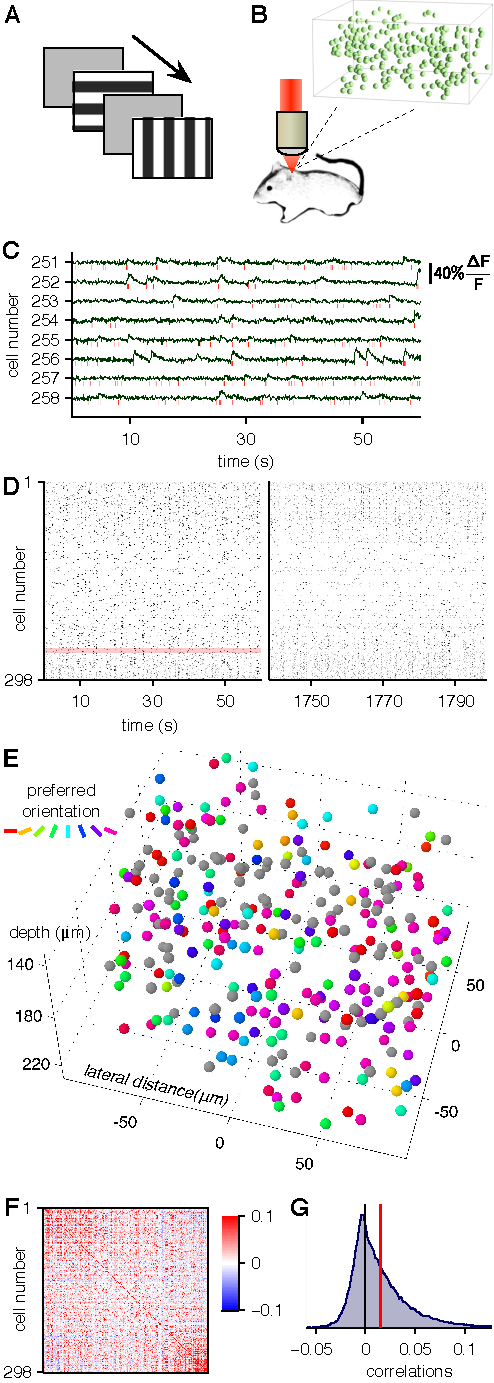
\includegraphics{figures/Acquisition.pdf}
\end{center}
\caption{
{\bf Acquistion of neural population activity using two-photon fluorescence imaging of calcium signal.}  {\sf A.} Visual stimuli comprising brief (500 ms) presentatios of full-field drifting gratings separated by blank screens. {\sf B.} Two-photon fast 3D imaging of calcium signals. {\sf D.} The first and last 30 seconds of a 30-minute recording of population calcium signals. The signals are deconvovled and binned at 150 ms. {\sf E.} The sample noise correlation matrix of neuronal calcium signals from {\sf D} after subtracting the average stimulus response. {\sf F.} The histogram of off-diagonal coefficients from the correlation matrix in {\bf D}.
}
\label{fig:01}
\end{figure}
